\documentclass{beamer}
\usepackage[american]{babel}
\usepackage{parskip}
\usepackage{pgfpages}
\usepackage{csquotes}
\usepackage{hyperref}

% \setbeameroption{hide notes} % Only slides
% \setbeameroption{show only notes} % Only notes
\setbeameroption{show notes on second screen=right} % Both

\title{Introducing Keto, the open source implementation of Zanzibar}
\author{Patrik Neu\\Open Source Maintainer @ Ory}
\date{\today}

\begin{document}
    \begin{frame}
        \titlepage

        \note[item]{breaking up hydra into separate services to not create yet another monolith trying to solve everything auth*}
        \note[item]{Keto first commit March 2018}
        \note[item]{Keto was build on open policy agent}
        \note[item]{from accumulating performance complains and our own experience we knew it was not a perfect fit}
        \note[item]{In 2019 at USENIX Google Research presented a paper about Google's internal authorization system, code-named Zanzibar.}
    \end{frame}

    \begin{frame}{Ory Design Philosophy}
        
        \begin{itemize}[<+->]
            \item 12 factor
            \item API service
            \item single compiled binary, minimal dependencies
            \item minimal size
            \item speed
        \end{itemize}

    \end{frame}

    \begin{frame}{Requirements for Zanzibar}

        \begin{itemize}[<+->]
            \item flexible
            \note<1>[item]{support all kinds of services, including Calendar, Cloud, Drive, Maps, Photos, and YouTube}
            \note<1>[item]{different data models and permission requirements}

            \item fast
            \item<.-> always available
            \note<2>[item]{authorization on critical path}
            \note<2>[item]{required for each and every request}
            \note<2>[item]{the best authorization system is never noticed by a regular user: don't feel overhead, don't experience errors}
            \note<2>[item]{applications such as search require many authorization checks to serve one result}

            \item consistent
            \note<3>[item]{false positives: fatal, users do stuff they are not allowed}
            \note<3>[item]{false negatives: at least annoying if time-bound, can be fatal if important tasks can not be done}

            \item Google scale
            \note<4>[item]{quote: "trillions of access control lists; millions of authorization requests per second"}
            \note<4>[item]{distributed across the globe}
            \note<4>[item]{cross-regional RTTs are already too high, handle locally}
        \end{itemize}

    \end{frame}

    \begin{frame}[fragile]{Zanzibar in 15 Minutes}{ACLs}

        \begin{itemize}[<+->]
            \item relation tuples
            \begin{verbatim}
files:cat.jpg#access@john
files:cat.jpg#access@(dirs:cats#access)
            \end{verbatim}

            \note<1>[item]{basic ACL structure}
            \note<1>[item]{namespace:object\#relation@subject}
            \note<1>[item]{translates to "john has access on the cat.jpg file"}
            \note<1>[item]{translates to "everyone who has access to the cats directory has access to the cat.jpg file"}

            \item subject set rewrites
            \note<2>[item]{defined globally in the namespace config}
            \note<2>[item]{case 1: automatically add tuples; examples: read if you have write}
            \note<2>[item]{case 2: compute effective set; examples: access child if access to parent, only access if you are admin AND got the explicit permission}
            \note<2>[item]{not yet implemented in Keto, but the next big thing to work on as they are important}

        \end{itemize}

    \end{frame}

    \begin{frame}{Zanzibar in 15 Minutes}{Graph of Relations}

        \begin{center}
            \href{https://mermaid-js.github.io/mermaid-live-editor/\#/edit/eyJjb2RlIjoiZ3JhcGggVERcbiAgICBzdWJncmFwaCBvYmogW09iamVjdCBSZWdpb25dXG4gICAgQVtjYXQuanBnXVxuICAgIEdbZG9nLmpwZ11cbiAgICBFW2NhdHNdIC0tPnxwYXJlbnR8IEFcbiAgICBIW2RvZ3NdIC0tPnxwYXJlbnR8IEdcbiAgICBlbmRcbiAgICBzdWJncmFwaCBzdWJqSUQgW1N1YmplY3QgUmVnaW9uXVxuICAgIEYoW3BldGVyXSlcbiAgICBDKFtqb2huXSlcbiAgICBlbmRcbiAgICBBIC0tPnxhY2Nlc3N8IEJ7e2NhdHMjYWNjZXNzfX1cbiAgICBBIC0tPnxhY2Nlc3N8IENcbiAgICBCIC0uIGNhdC5qcGcjYWNjZXNzIC4tPiBGXG4gICAgRSAtLT58YWNjZXNzfCBGXG4gICAgRyAtLT58YWNjZXNzfCBGXG4iLCJtZXJtYWlkIjp7fSwidXBkYXRlRWRpdG9yIjpmYWxzZX0}
            {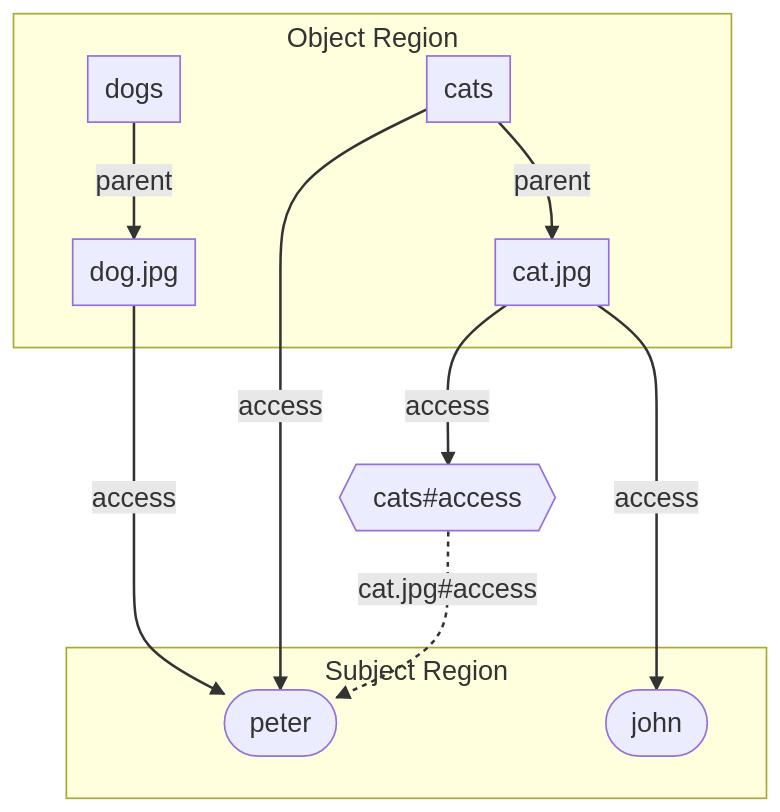
\includegraphics[height=0.8\textheight]{graph-of-relations.png}}
        \end{center}

        \note[item]{not only neat to look at}
        \note[item]{graph algorithms are well studied and common}
        \note[item]{ACL check $\equiv$ reachability of node}
        \note[item]{Expand subject set by some graph traversal algorithm}
        \note[item]{relation tuples will usually result in a clustered/structured graph}
        \note[item]{relation tuples are directed edges}

    \end{frame}

    \begin{frame}{Zanzibar in 15 Minutes}{Zookies}

        Consistency, latency, availability - choose any three?

        \note<1>[item]{background in distributed systems}
        \note<1>[item]{research and theorems show that requirements are in conflict}
        \note<1>[item]{all can be meet at the same time once data are propagated}
        \note<1>[item]{determine whether local data are recent enough}

        \pause

        \begin{itemize}[<+->]
            \item encode object version (timestamp)
            \note<2>[item]{distributed systems: clock synchronisation is very hard}
            \note<2>[item]{real-time easy for Google: GPS in datacenters to sync clocks}

            \item stored next to object and provided in every request
            \note<3>[item]{Local cache ACLs have to be at least as recent as object version}
            
            \begin{itemize}
                \item subject previously had permission $\Rightarrow$ might still access object versions it already had access to
                \note<4>[item]{only during propagation time}
                \note<4>[item]{new object versions will always be rejected}
                
                \item subject newly got permission $\Rightarrow$ might temporarily not have access to previous object versions
                \note<5>[item]{only during propagation time}
                \note<5>[item]{new object versions will always be allowed}
            \end{itemize}

            \item idea for Keto: logical clock based on bloom filters
            \note<6>[item]{zookies not yet implemented (only single node operation)}
            \note<6>[item]{bloom filter based to allow dynamic number of nodes}
            \note<6>[item]{not settled, still searching for ideas}

        \end{itemize}

    \end{frame}

    \begin{frame}{Current State of Keto}

        \begin{itemize}[<+->]
            \item single node operation mode (scaling horizontally possible)
            \item read, write, check, and expand APIs
        \end{itemize}

        \only<3->{Next steps:}

        \begin{itemize}[<+->]
            \item subject set rewrites
            \item zookies
            \item native ABAC \& RBAC support
            \item integration with wider authorization ecosystem
            \item heavy caching \& cluster mode
        \end{itemize}

    \end{frame}

    \begin{frame}{How we got here}

        \begin{itemize}[<+->]
            \item announce deprecation of OPA-Keto early on
            \note<1>[item]{multiple channels}
            \note<1>[item]{no migration path yet}

            \item transparently document all work
            \note<2>{instead of developing in the dark and suddenly pushing the new version}

            \item valuable input and contributions from our lovely community
            \note<3>[item]{although git shows that I did most work}
            \note<3>[item]{ideas were always discussed with multiple people}
            \note<3>[item]{community members followed me into the rabbit hole}
            \note<3>[item]{jumped on calls to discuss details, ideas and findings}
            
            \item idea behind zanzibar is minimalistic
            \note<4>[item]{check engine currently 39 LoC}

        \end{itemize}

    \end{frame}

    \begin{frame}{Open Source Foundation}

        \note[item]{like our other open source projects}
        \note[item]{}
        
        \begin{itemize}
            \item Go
            \item gRPC
            \item OpenAPI Spec
            \item gobuffalo/pop
            \item Cobra
            \item Docusaurus
            \item Docker
        \end{itemize}

    \end{frame}

    \begin{frame}{First Learnings}

        \note[item]{from our own SaaS cloud production system}
        \note[item]{from community feedback}

        \begin{itemize}[<+->]
            \item as flexible as anticipated
            \item subject set rewrites are \textbf{very} important
            \item gRPC \& REST interfaces are both valuable
            \item databases are good at handling few huge tables
            \item relation tuples are not straight forward to design
        \end{itemize}

    \end{frame}

    \begin{frame}{Link Collection}

        \begin{itemize}
            \item \href{https://github.com/ory/keto}{Keto on GitHub}
            \item \href{https://www.ory.sh/keto/docs/quickstart}{Keto Quickstart Tutorial}
            \item \href{https://slack.ory.sh/}{Ory Community Slack}
            \item \href{https://research.google/pubs/pub48190/}{Zanzibar Paper}
            \item \href{mailto:patrik@ory.sh}{My email: patrik@ory.sh}
        \end{itemize}

    \end{frame}

\end{document}
